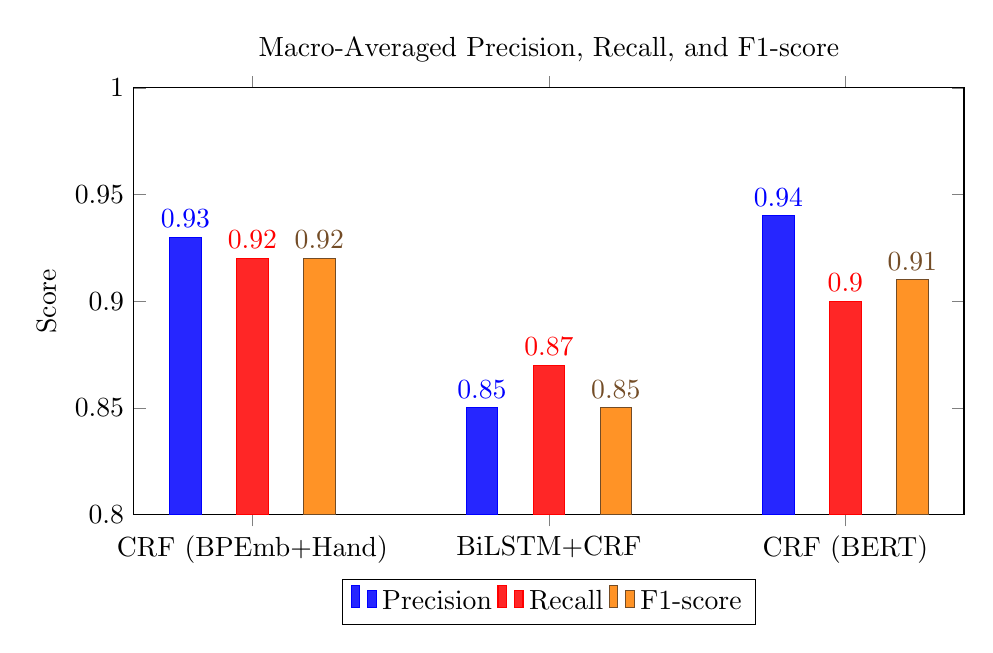
\begin{tikzpicture}  
    % Bar chart data
    \begin{axis}[
        ybar,
        bar width=.40cm,
        width=\textwidth,
        height=7cm,
        enlarge x limits=0.2,
        ylabel={Score},
        ymin=0.80, ymax=1.0,
        symbolic x coords={CRF (BPEmb+Hand), BiLSTM+CRF, CRF (BERT)},
        xtick=data,
        nodes near coords,
        nodes near coords align={vertical},
        legend style={at={(0.5,-0.15)}, anchor=north, legend columns=-1},
        xlabel={Model},
        title={Macro-Averaged Precision, Recall, and F1-score},
    ]
    \addplot+[style={fill=blue!85}, bar shift=-0.85cm] coordinates {
        (CRF (BPEmb+Hand),0.93) 
        (BiLSTM+CRF,0.85) 
        (CRF (BERT),0.94)
    };
    \addplot+[style={fill=red!85}, bar shift=0cm] coordinates {
        (CRF (BPEmb+Hand),0.92) 
        (BiLSTM+CRF,0.87) 
        (CRF (BERT),0.90)
    };
    \addplot+[style={fill=orange!85}, bar shift=0.85cm] coordinates {
        (CRF (BPEmb+Hand),0.92) 
        (BiLSTM+CRF,0.85) 
        (CRF (BERT),0.91)
    };

    \legend{Precision, Recall, F1-score}
    \end{axis}
\end{tikzpicture}